%==============================================================================
% ANEXOS
%==============================================================================
% Un solo anexo de figuras complementarias: la separación energía-tiempo por nivel
% de frecuencia (antes solo en el material complementario, docs/libro/README.md,
% sección 7) y las figuras de apoyo de los clasificadores, movidas desde Resultados.

\appendix
\renewcommand{\appendixname}{Anexo}
\renewcommand{\thefigure}{\Alph{chapter}.\arabic{figure}}

\chapter{Figuras complementarias}
\label{cap:anexo-figuras}

Las dos primeras figuras separan en energía y tiempo el EDP de cada nivel de frecuencia de la Fase 1, y muestran por qué la política de CPU es \textit{no actuar} en ambas clases y por qué la de GPU fija F1 en \textit{memory\_bound} (secciones \ref{sec:resultados-cpu-politica} y \ref{sec:resultados-gpu-politica}). La tercera muestra los perfiles gemelos entre clases opuestas que limitan al clasificador de CPU (sección \ref{sec:resultados-cpu-final}), y la cuarta, la auditoría de invarianza que eligió el modelo de GPU desplegado (sección \ref{sec:resultados-gpu-invarianza}).

\begin{figure}[H]
    \centering
    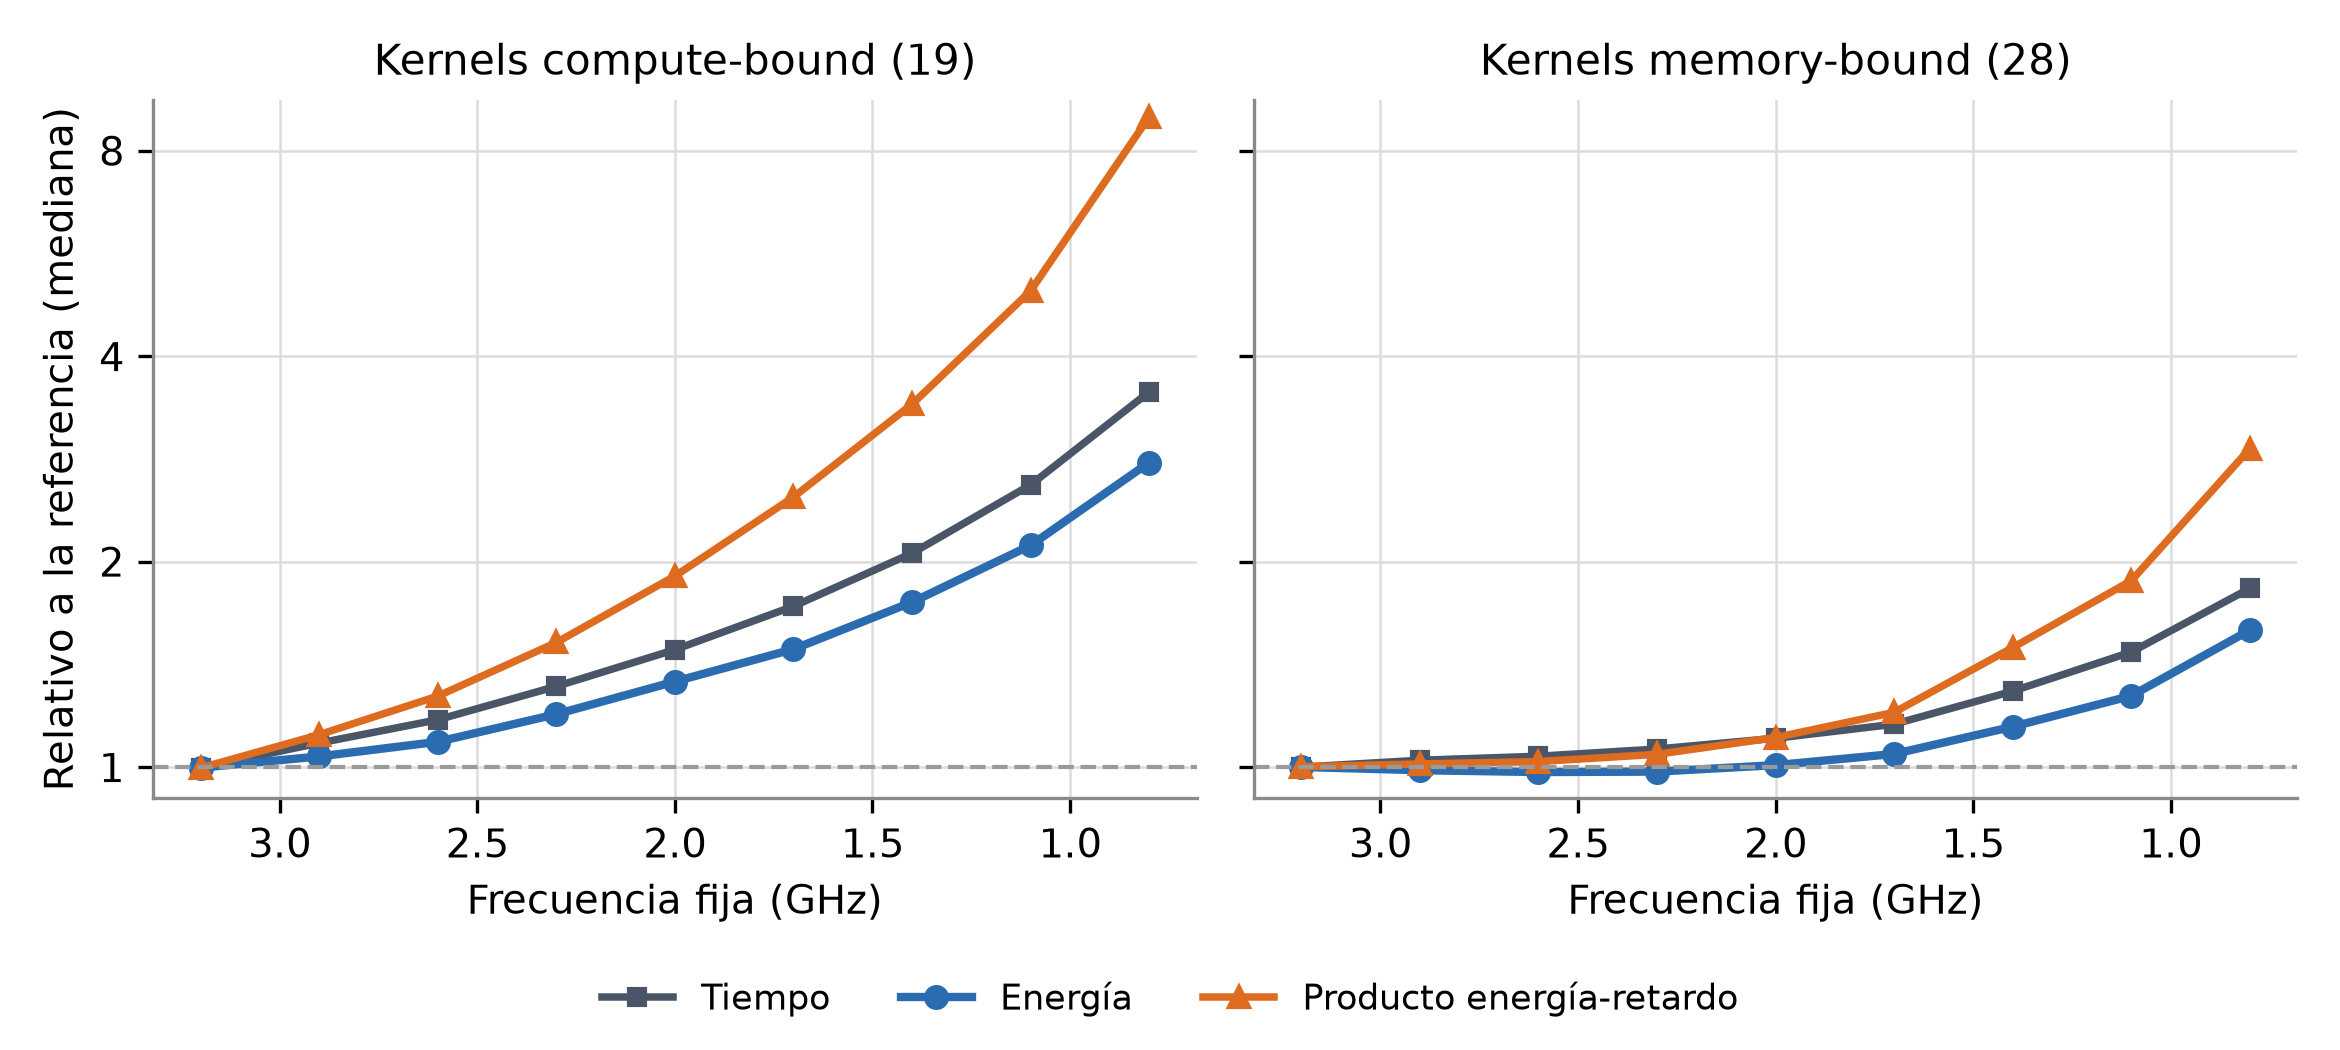
\includegraphics[width=0.85\textwidth]{figuras/fig_cpu_energia_relativa_20260920.png}
    \caption[Energía, tiempo y EDP por nivel de frecuencia en CPU]{Mediana entre kernels de la energía (paquete y DRAM), el tiempo y el EDP de cada nivel fijo de CPU, relativos a la referencia nativa, para las dos clases. El eje vertical es logarítmico. Fuente: elaboración propia.}
    \label{fig:anexo-cpu-energia-relativa}
\end{figure}

\begin{figure}[H]
    \centering
    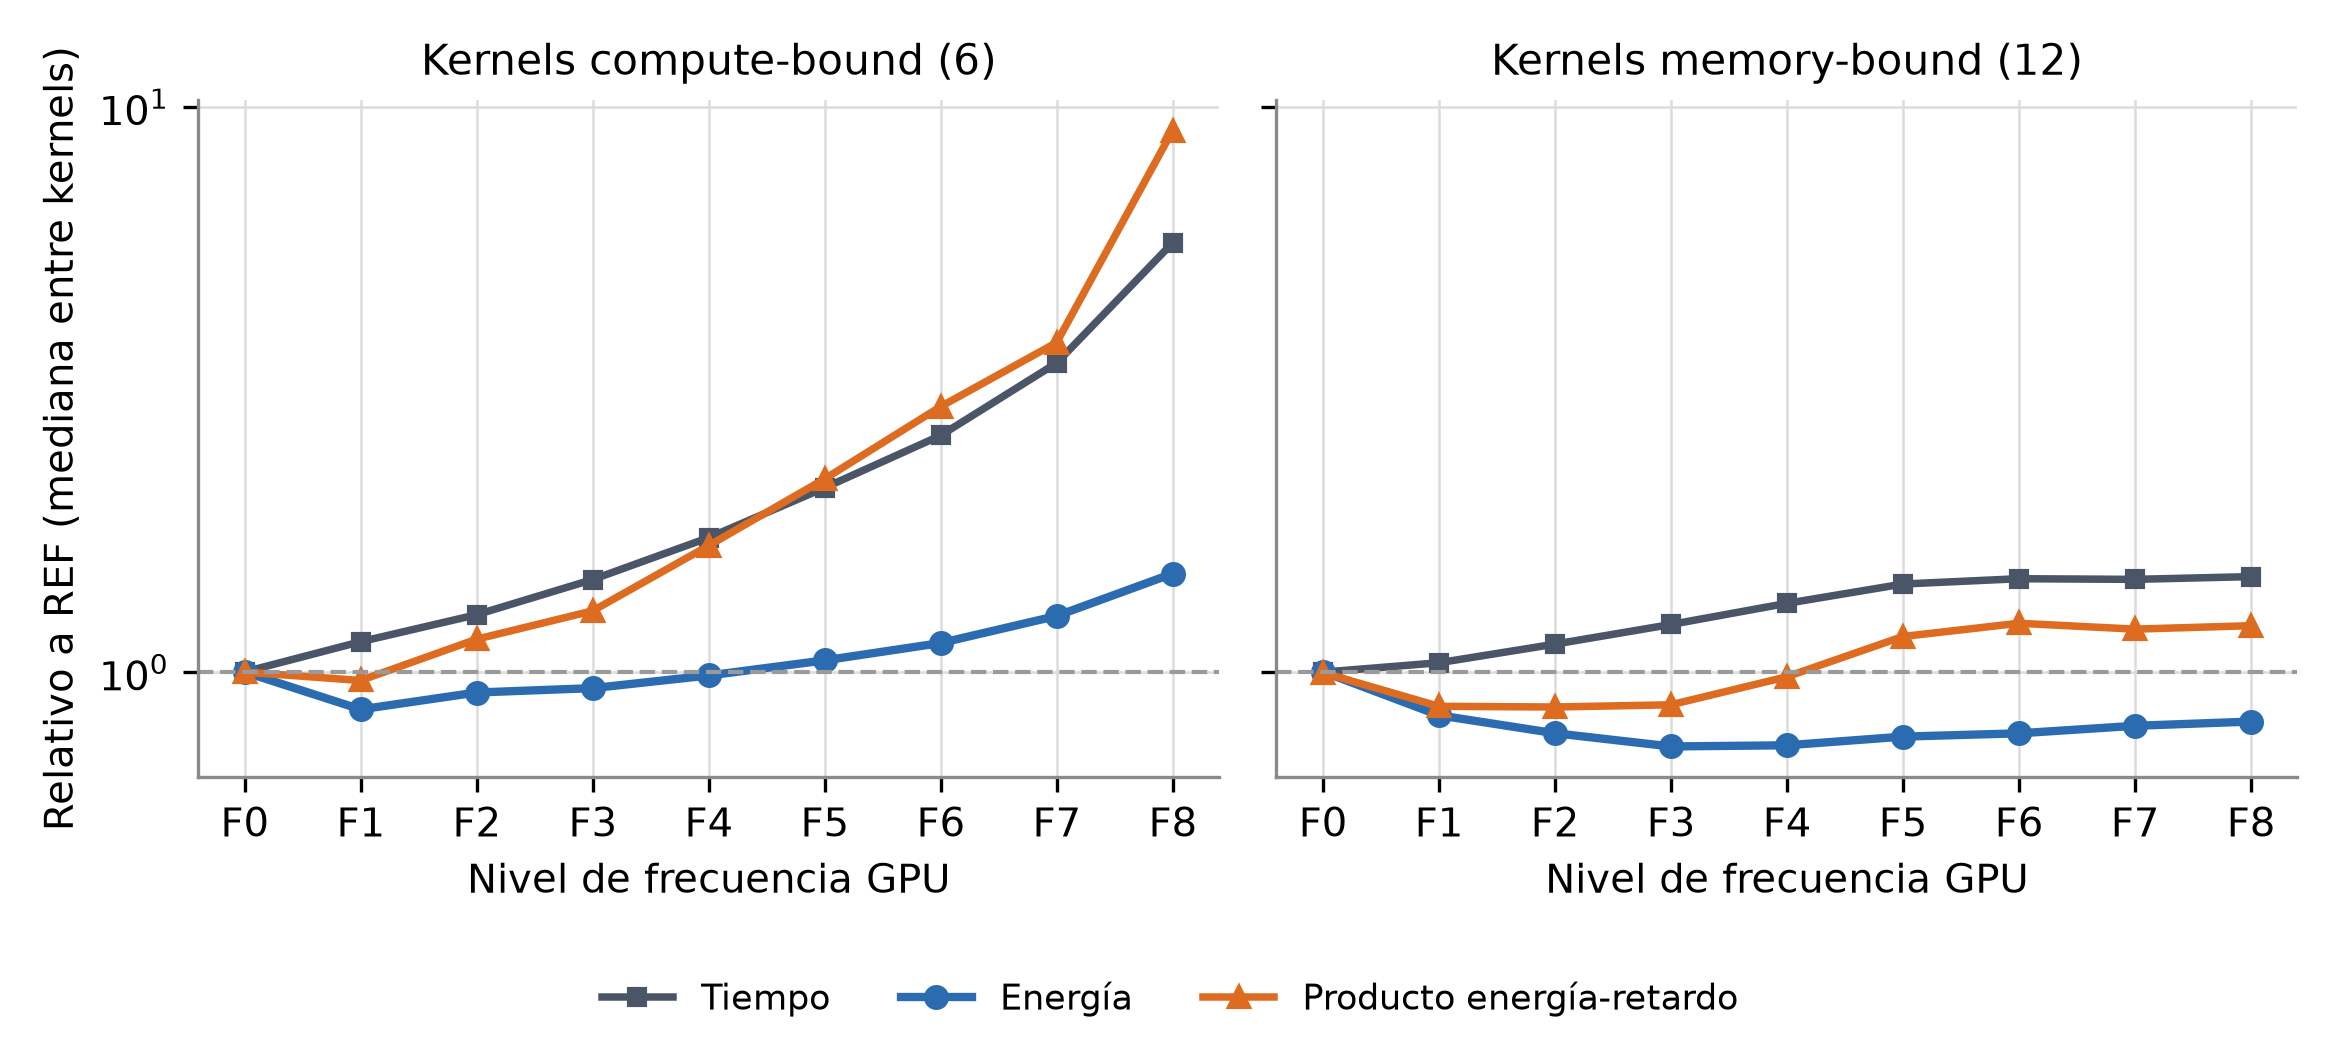
\includegraphics[width=0.85\textwidth]{figuras/fig_gpu_politica_energia_relativa_20260922.png}
    \caption[Energía, tiempo y EDP por nivel de frecuencia en GPU]{Mediana entre kernels del tiempo, la energía y el EDP de cada nivel de reloj de GPU, relativos a la base, para las dos clases (5 y 9 kernels con corridas en la base, kernel como unidad, descriptivo). El eje vertical es logarítmico. Fuente: elaboración propia.}
    \label{fig:anexo-gpu-energia-relativa}
\end{figure}

\begin{figure}[H]
    \centering
    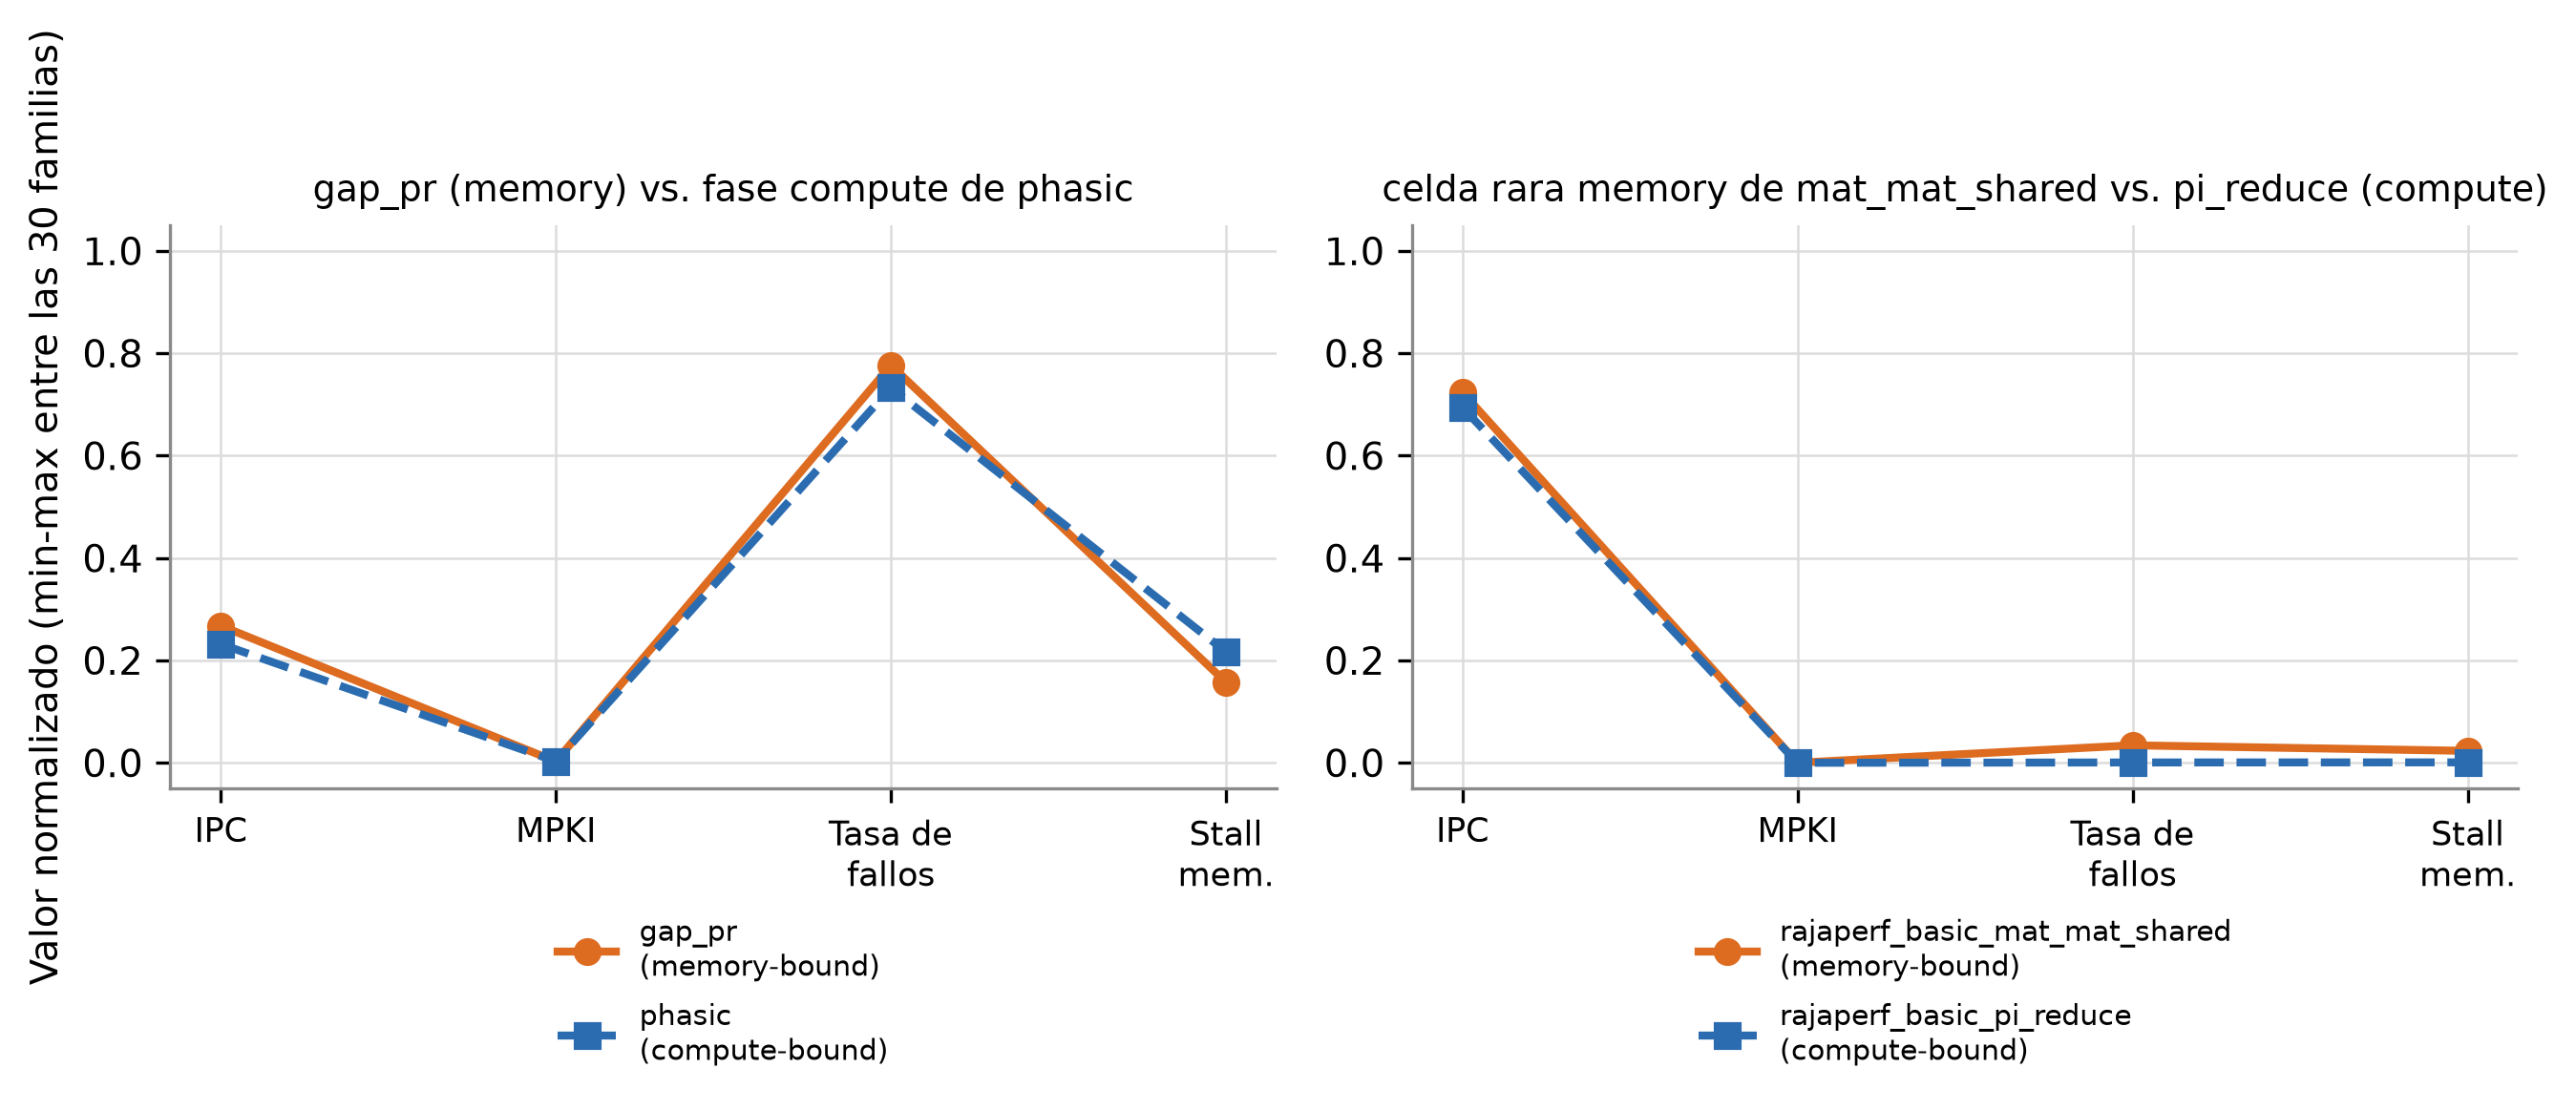
\includegraphics[width=0.96\textwidth]{figuras/fig_cpu_perfiles_gemelos_20260922.png}
    \caption[Perfiles de celdas confusables entre clases opuestas]{Cuatro variables de entrada, normalizadas al rango de las 30 familias, para los dos pares de celdas más confusables entre clases opuestas. Fuente: elaboración propia.}
    \label{fig:cpu-perfiles-gemelos}
\end{figure}

\begin{figure}[H]
    \centering
    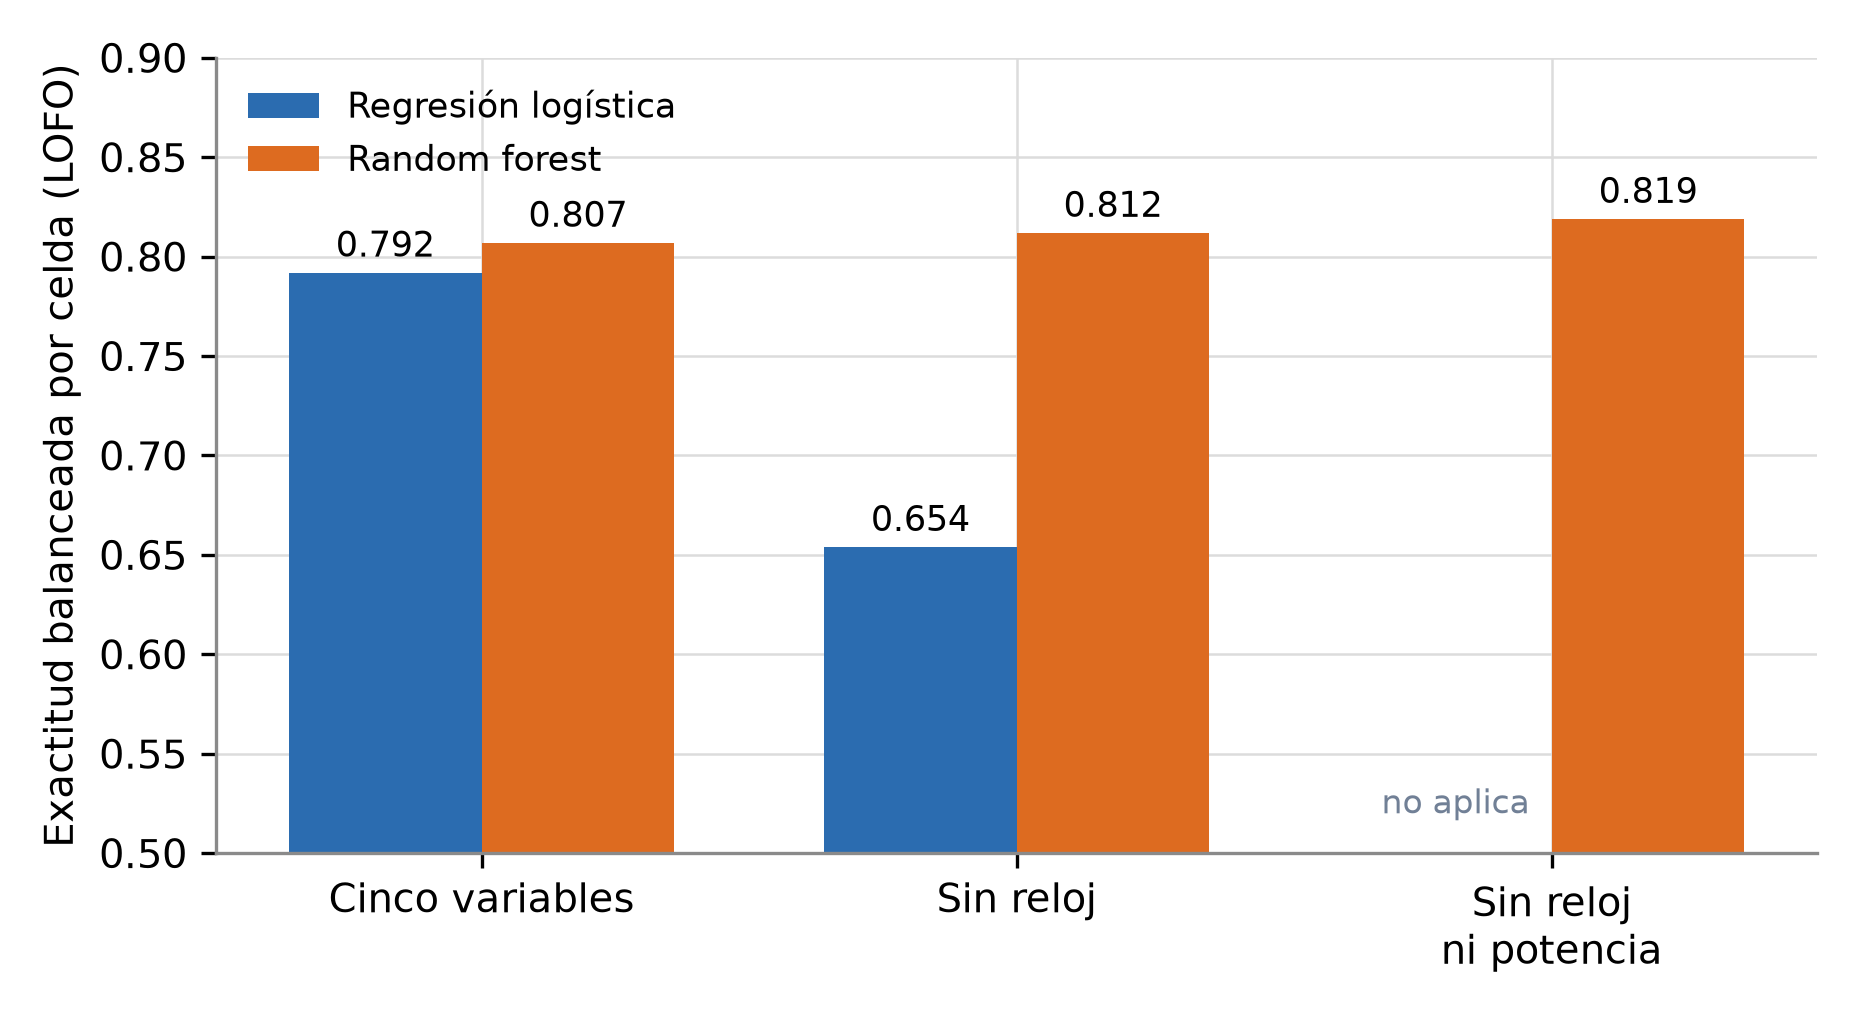
\includegraphics[width=0.70\textwidth]{figuras/fig_gpu_invarianza_reloj_20260923.png}
    \caption[Invarianza de los candidatos GPU frente al reloj]{Exactitud balanceada por celda (LOFO, 483 corridas, 16 familias) al excluir las variables que dependen de la acción del agente. Fuente: elaboración propia.}
    \label{fig:gpu-invarianza}
\end{figure}
